\subsubsection{Wrapper Methods}
\label{sec:methods.flat.wrapper}

% Author: Silvana

In contrast to filter methods, wrapper methods consider the properties of the classifier which will be used for classification.
The feature-set is selected so that it fits the biases and heuristics of the classifier as good as possible. 

Wrapper methods basically perform the following two steps iteratively: 

\begin{itemize}
  \item Search: A search routine selects a set of features 
  \item Evaluation: The selected subset is evaluated with the desired classifier
\end{itemize}

The search and evaluation steps are repeated until a stopping criterion is met, for example when a desired quality of classification is reached, 
or until a maximum number of iterations was performed. The subset which performed best is selected to train the actual classifier,
and normally, another evaluation with an independent testing set is done before actually using it for classification.
(See figure ~\ref{fig:methods.flat.wrapper.diagramm}) 

\begin{figure}[!ht]
  \centering 
  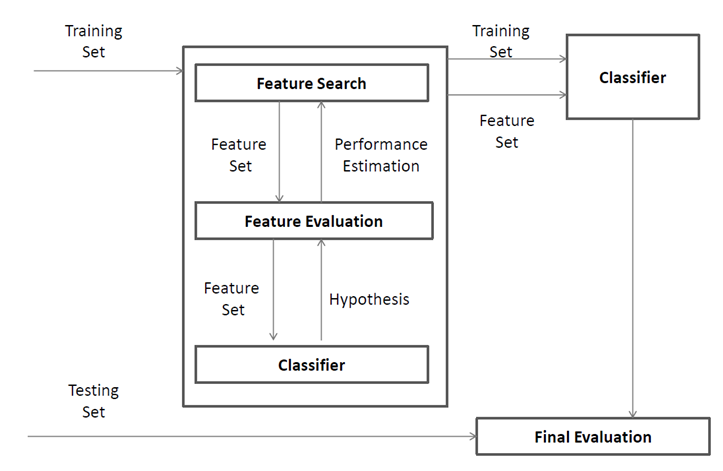
\includegraphics[width=0.8\textwidth]{chapters/methods/flat/wrapper_diagramm}
  \caption{Reprinted from \cite{Tang:04}. Basic scheme of a wrapper method. Using a training set, search and evaluation steps are performed iteratively.
	The search-algorithm provides potential feature-subsets which are evaluated by actually training the classifier. The quality is either heuristically estimated
	or evaluated by cross validation. After a stopping criterion is met, the actual classifier is trained and evaluated with an independent testing set again before
	being used for the actual classification task.}
  \label{fig:methods.flat.wrapper.diagramm}
\end{figure}

When choosing a search routine, the structure and size of the search space should be taken into account. As the feature space in the majority of 
applications is high dimensional, it is not possible to enumerate all possible feature subsets. Greedy algorithms are a popular choice,
but tend to get stuck in local optima when exploring big search spaces. in contrary, genetic algorithms are more complex, but are more likely
to explore the search space thoroughly and find a global optimum.

When a potential subset is found, its performance for the desired classifier has to be evaluated. 
This can be done for example by simply using a validation set, or by performing cross-validation.

The major drawback of wrapper methods is the computation time needed, as the subsequent search- and evaluation steps are computationally expensive: 
Every time a potential feature subset is selected, the classifier has actually to be trained with a training set and evaluated (for example by performing
cross validation, or using accuracy estimation.\cite{Kohavi:97}) Because the finally selected subset is dependent on the classification algorithm, 
it will eventually produce biased results when being used with an arbitrary classifier. 

Compared to filter methods, wrapper methods have the big advantage of selecting feature subsets which normally produce more accurate classification results.
Their better performance thus justifies the long computation time.

This next chapters will go more in-depth about the different search-techniques. First, the general strategies forward selection and backwards elimination 
are introduced, then search by greedy algorithms and genetic algorithms are explained in more detail.

\paragraph{Forward Selection/backward elimination}
\label{par:methods.flat.wrapper.forward_selection}

% Author: Silvana
In practice, two methods which are often used for large data sets are sequential forward selection (SFS) and sequential backward elimination (SBE).
 
Both  technique work  iteratively. Forward selection starts with an empty set, where no feature is selected in the beginning. 
Sequentially, one  feature after the other is added to the subset, so that the new subset maximizes the quality of  the  subset,
which is measured by some criterion function J. This is done until the set has reached a desired size. SBE works exactly the other way round, 
starting with the full set of features first and sequentially deleting features, until a smaller subset of sufficient quality is gained. 

Both methods have a major drawback: Either features cannot be eliminated once they have been selected (SFS), 
or they cannot be selected again if they have been discarded once (SBE). The assumption, that the best five selected features  must contain a 
subset of the best four selected features does not hold in practice. \cite{Nakariyakul:08}

\cite{Pudil:94} proposes Sequential forward floating selection as improvement (and, respectively, Selective backward floating elimination). 
A backtracking step is implemented after each sequential addition or deletion, which tries to find eventually better subsets. Both methods 
show admissible computation-time for small- or medium scaled problems, and perform better than other sequential methods on a variety of
problems. However, it should be empathized that they do not always perform better than other methods, but at least "good enough" on the 
majority of problems. For very big datasets, they are outperformed by genetic algorithms. \cite{Kudo:00}   

\cite{Mao:04} proposes \textit{orthogonal} forward selection and backward elimination to overcome problems that occur with SFS and SBE. 
Instead of simply selecting features in a sequential way, they are first mapped to an orthogonal space. 
This mapping decorrelates the features, so they can be evaluated and selected individually. 
After the selection, the features are linked back to the same number of variables in the original measurement space.
Using a mapping to orthogonal space proved to be very effective for features with high correlation. 
If the correlation between candidate features is only trivial, orthogonal
transforms don't improve the results compared to existing sequential methods.
\paragraph{Hill Climbing}
\label{par:methods.flat.wrapper.hill_climbing}

% Author: Silvana

Hill climbing, sometimes also referred to as "steepest ascend", is probably the simplest search technique that can be applied. Starting with no features at all, an evaluation function rates the available features and adds the most relevant one to the subset. Then the procedure is repeated, each time adding the most relevant feature of the remaining set to the subset. As soon as the influence of an added feature does not improve the overall quality of the set significantly, the search is stopped. The problem with hill climbing is that it gets stuck in local maxima easily, and fails in finding a globally optimal solution. \cite{Kohavi:97}

Best-first search outperforms hill-climbing and turns out to be a more robust technique according to Kohvani \cite{Kohavi:97}.
%\paragraph{Best First}
\label{par:methods.flat.wrapper.best_first}

% Author: Silvana
  
Best-first search outperforms hill-climbing, as it is a more robust technique. \cite{Kohavi:97} --Only one sentence and mentioned with hill climbing
\paragraph{Branch and Bound}
\label{par:methods.flat.wrapper.branch_and_bound}

% Author: Silvana

Branch-and-bound (BB) is a general design principle for solving discrete and combinatorial optimization problems. BB-algorithms work by building up a search tree with possible candidate solutions (branch phase). Further, a criterion function has to be designed, which evaluates the "quality" of possible solutions represented by nodes in the tree. Then, the branches of the tree are explored to find a global optimum for the given function. To avoid that the search is exploring the whole possible space, and thus degenerating to a brute-force-approach, it is limited by so-called bounds, which prune the tree when it becomes unlikely to find an optimum in the current branch. 

For feature selection, Narendra et al. \cite{Narendra:77} first proposed a BB-algorithm based on efficient subset selection. The root of the tree represents the full set of features, whereas leaf-nodes represent single features (or subsets of the smallest desired size). Monotonicity is required regarding the criterion function and the subsets. That means, if a current subset is below a bound, then its following child nodes are assumed to be also lower than that bound. Thus, the search in this particular branch can be aborted, and continued at another branch. Additionally, the sorting of the nodes is done with an efficient enumeration scheme to augment finding an optimal solution in a short amount of time.

The problem with BB-methods is that it is not guaranteed to perform better (faster) than exhaustive search methods. It is not granted that enough sub-trees will be pruned to speed up the search sufficiently, in worst-case, the criterion-function is evaluated for every node in the tree. Additionally, evaluating the function close to the root takes longer than evaluating it at the leaves. \cite{Somol:04} proposed a fast BB approach, which tries to keep the evaluations of the criterion function at a minimum to speed up the search. The algorithm is "learning" how the removal of features influences the functions value, and tries to "predict" changes without doing the actual computation. Only if the predicted value comes close to a bound, the criterion function is evaluated, otherwise the algorithm continues descending in the tree.

Adaptive branch and bound for feature selection \cite{Nakariyakul:07} also tries to reduce the number of evaluations of the criterion function, by applying several improvements. Already when building up the tree, the order of the nodes corresponds to the importance of the features. Then, instead of trying to descend sequentially from node to node, an adaptive, "jumping" search method is used to avoid more-or less redundant computations of the evaluation function. Additionally, the initial bound used in the search and also the initial search level are chosen in an optimal way. (Comment: only tested on 30 features?! Still check this out...)

\paragraph{Genetic Algorithms}
\label{par:methods.flat.wrapper.genetic}

% Author: Silvana

(SOURCE!!! basically written down by what Silvana knows from se bachelor thesis...)
Before explaining how GA can be used for for feature selection, 
a short introduction into the very basic concept of those algorithms has to be made. As the name implies, 
genetic algorithms are inspired by the way nature �works� in real life: parents carry specific genetic  information, 
and a (re-)combination of this information is passed to their kids in order to create �better� offspring from generation to generation. 
GA's imitate this behaviour by encoding the data they should work on or optimize in so-called chromosomes 
(which could be for examples vectors of numerical values). 
One is not limited to using numerical data, but this is a very common approach, 
as numerical values can be processed easily by the typical routines in a GA. 
A desired number of chromosomes is initialized at the beginning of the algorithm. 
They can be created randomly (f.ex by creating vectors with random values) or according to specific rules.
As the algorithm starts, different operations are applied to create new chromosomes: 
for example, a new chromosome can be obtained by combining the values of two already existing chromosomes, 
or by changing random values in an already existing chromosome. 

The resulting new chromosomes are then evaluated according to a fitness function, 
which basically measures how �good� a chromosome is suited for the underlying problem. 
The chromosomes then can be ranked, and the best ones are taken again to create new offspring. 
This procedure is repeated as long until a desired quality/result is achieved.

Just like branch and bound algorithms, GA are generally not suited for big feature spaces, 
as they try to explore the whole search space until a stopping criterion is met. 
This takes a lot of computation time when feature spaces are highly dimensional. 
The strength of GA is that they do not tend to get stuck at local optima 
(es for example Hill climbing algorithms do), but instead are likely to find global optima.

For feature selection, the chromosomes could correspond to subsets of the total feature set. 
The values in a chromosome would encode if a feature is selected or not. This can be achieved simply by using binary values: 
1 indicates that a feature is selected for a possible subset, and 0 indicates that it is not selected. 
Mutation and recombination operators would modify the chromosomes, 
and a fitness function would evaluate their quality for the underlying classifier 
(remember, each chromosome resembles a subset of features).

But one is not limited to binary values [XY] and [BLA] used GA to find optimal kernel setting for SVM. [quote those two papers found from  2006] 

  
TODO
Bla bla bla\ldots
